%%%%%%%%%%%%%%%%%%%%%%%%%%%%%%%%%%%%%%%%%
% Original author:
% Linux and Unix Users Group at Virginia Tech Wiki
% (https://vtluug.org/wiki/Example_LaTeX_chem_lab_report)
% Modified by: Hector F. Jimenez S, for the Digital Electronics Laboratory.
% License:
% CC BY-NC-SA 3.0 
%%%%%%%%%%%%%%%%%%%%%%%%%%%%%%%%%%%%%%%%%
%----------------------------------------
%	PACKAGES AND DOCUMENT CONFIGURATIONS
%---------------------------------------
\documentclass[paper=a4, fontsize=12pt]{article} 		% A4 paper and 11pt font size
\usepackage[T1]{fontenc} 								% Use 8-bit encoding that has 256 glyphs
%\usepackage{fourier}		 							% Use the Adobe Utopia font for the document 
\usepackage[spanish,english]{babel}						% Spanish Language, templates uses some sections in english.
\selectlanguage{spanish}								% main language.
\usepackage[utf8]{inputenc}								% tildes for spanish language.
\usepackage{amsmath,amsfonts,amsthm} 					% Math packages.
\usepackage{lipsum} 									% inserting dummy 'Lorem ipsum' text into the template
\usepackage{minted}
\usepackage{sectsty} 									% Allows customizing section commands
\allsectionsfont{\centering \normalfont\scshape}	   	% Make all sections centered, the default font and small caps
\usepackage{hyperref}
\hypersetup{											%Setups the false color and borders.
    colorlinks=false,
    pdfborder={0 0 0},
}
\newcommand\fnurl[2]{%									% set a simple and quick footnote command and include url.
\href{#2}{#1}\footnote{\url{#2}}%	
}
\usepackage{graphicx}									%Import easyly images.
\graphicspath{ {./images/} }							%Where to look for the images.
\DeclareGraphicsExtensions{.pdf,.png,.jpg}
\usepackage[notes,backend=biber]{biblatex-chicago}
\bibliography{biblio}
\usepackage{fancyhdr} 									% Custom headers and footers
\pagestyle{fancyplain} 									% Makes all pages in the document conform to the custom headers and footers
\fancyhead{} 											% No page header - if you want one, create it in the same way as the footers below
\fancyfoot[L]{} 										% Empty left footer
\fancyfoot[C]{} 										% Empty center footer
\fancyfoot[R]{\thepage} 								% Page numbering for right footer
\renewcommand{\headrulewidth}{0pt} 						% Remove header underlines
\renewcommand{\footrulewidth}{0pt} 						% Remove footer underlines
\setlength{\headheight}{13.6pt} 					    % Customize the height of the header
\numberwithin{equation}{section}						% Number equations within sections (i.e. 1.1, 1.2, 2.1, 2.2 instead of 1, 2, 3, 4)
\numberwithin{figure}{section} 							% Number figures within sections (i.e. 1.1, 1.2, 2.1, 2.2 instead of 1, 2, 3, 4)
\numberwithin{table}{section} 							% Number tables within sections (i.e. 1.1, 1.2, 2.1, 2.2 instead of 1, 2, 3, 4)

\setlength\parindent{0pt} 								% Removes all indentation from paragraphs

%----------------------------------------
%	TITLE SECTION
%----------------------------------------
\newcommand{\horrule}[1]{\rule{\linewidth}{#1}} 		% Create horizontal rule command with 1 argument of height

\title{Desarrollo de un Controlador de Tráfico\\ 
Usando FPGA's \\
Laboratorio de Electrónica Digital\\Módulo: 1} 			% Title

%\horrule{0.5pt} \\[0.4cm] 								% Thin top horizontal rule	Title rule
%\huge Assignment Title \\ 								% The assignment title
%\horrule{2pt} \\[0.5cm] 								% Thick bottom horizontal rule
\author{
Héctor F. \textsc{Jiménez Saldarriaga}\\
\texttt{hfjimenez@utp.edu.co} \\
\texttt{PGP KEY ID: 0xB05AD7B8}
\and
Steffany \textsc{Lopez Segura}\\
\texttt{steffany@utp.edu.co}
}        %End of  Author name
\date{}    						                       % Date for the report
\begin{document}
\maketitle                      			           % Insert the title, author and date
\begin{center}
\begin{tabular}{l r}
Fecha de Entrega: & Febrero 24, 2016 \\				   % Ramiro's Details.
Profesor: & Ing.Msc(c) Ramiro Andres Barrios Valencia
\end{tabular}
\end{center}
%%%%%%%%%%%	
% Let's start the document.
%%%%%%%%%%%	
\section{Objectivos}
\begin{itemize}
  \item Fortalecer y poner en práctica la teoria de circuitos combinacionales.
  \item Fortalecer el desarrllo de sistemas digitales, utilizando el lenguaje \emph{VHDL} y el entorno de desarrollo Xilinx ISE.
  \item Identificar la arquitectura, esquematicos y hardware integrado de la placa de desarrollo \emph{NEXYS2}.
  \item Implementar en lenguaje VHDL un módulo que permita la detección correcta de los pulsos entregados por los botones presentes en la tarjeta de desarrollo\footnote{Datasheet Oficial de la placa  Nexys 2 \fnurl{Manual}{http://reference.digilentinc.com/_media/nexys:nexys2:nexys2_rm.pdf}}
  \item Identificar posibles problemas a la hora de acoplarnos con los otros módulos a desarrollar.
\end{itemize}

%%%%%%%%%%%	
% Theory Marc! 
%%%%%%%%%%%	
\section{Marco Teórico}
\label{sec:problemamecanico}
Utilizar switches y pulsadores mecánicos en un sistema electrónico es una práctica muy común, pues sirven de interface entre el usuario y el sistema embebido para seleccionar y programar opciones que este posee; en la práctica actual muchos de estos sistemas mecánicos están siendo reemplazados por displays táctiles pero hay situaciones industriales principalmente en las cuales un pulsador mecánico sería una solución mas apropiada y eficiente en la implementación, pues al ser sistemas mecánicos estos no se degradan tan rápido como lo harían las pantallas táctiles. Una de las grandes desventajas que poseen los pulsadores son los rebotes, los elementos mecánicos del pulsador son elásticos, esto hace que cuando pulsemos o despulsemos, haya un instante en el que se realicen varios contactos seguidos, además de una barrera o GAP que se produce por el aire allí\textit{(típicamente es despreciable por su baja fuerza discipativa )} que existen entre los elementos elásticos, esto puede inducir múltiples pulsaciones, flancos y falsas señales instantáneamente, ocasionando un mal funcionamiento del dispositivo.
Existen muchas formas de lidiar con este problema, tanto soluciones por hardware físico o por software como lo realizaremos en este reporte, mediante la implementación de un circuito lógico provisto por la empresa \fnurl{Digikey}{http://www.digikey.com/}
%%%

En definitiva, se trata de un mecanismo simple (los hay muy sofisticados), constituido por un par de contactos eléctricos que se unen o separan por medios mecánicos. En electricidad, los falsos contactos que se producen el ser utilizados normalmente, en algunos casos produce una chispa debido a la corriente que atraviesa los contactos, provocando que quemen en parte y ennegreciendo los contactos eléctricos, lo que a la larga acaba deteriorando dichos contactos. La chispa se produce siempre al separar los contactos (desconectar), en ocasiones parece que también salta al conectarlos, eso es debido a los rebotes mecánicos que se producen al cambiar de estado.

Esto que en electricidad se considera normal, en electrónica es un verdadero nido de problemas, debido a dichos falsos contactos. Por su propia naturaleza, al cambiar de posición un interruptor, los contactos chocan entre sí y esto significa una serie de falsos contactos que se reproducen de un modo sin control, por lo que se generan los temidos rebotes (debounce en inglés), estos rebotes, se producen incluso cuando unimos dos cables desnudos, simulando un interruptor o pulsador.

%%
Los problemas 
\section{Arquitectura del la Placa \emph{NEXYS 2}}
La tarjeta de entrenamiento \emph{NEXYS 2} es una plataforma de desarrollo fabricada por la empresa \footnote{Digilentinc Pagina Oficial \fnurl{Nexys2 Spartan3E}{http://store.digilentinc.com/nexys-2-spartan-3e-fpga-trainer-board-retired-see-nexys-4-ddr/}} aunque se encuentra descontinuada para la venta y recomiendan utilizar esta misma en su version \textbf{4}, utiliza una fpga Spartan 3E optimizada para desarrollo de aplicaciones donde se requiere implementar diseños de lógica compleja, e ideal para el procesamiento de señales y desarrollo de sistemas embebidos como se menciona en \fnurl{General Spartan Versions}{http://www.xilinx.com/support/documentation-navigation/silicon-devices/mature-products/spartan-3e.html}, \fnurl{Spartan-3E FPGA Family: Introduction and Ordering Information}{http://www.xilinx.com/support/documentation/data_sheets/ds312.pdf}.
\\Algunos elementos destacables de la placa son :
\begin{description}
  \item[Connectores] \hfill \\
  	\begin{itemize}
		\item Puerto USB2.0
	    \item Puerto VGA
		\item PS/2
	    \item Puerto RS232
    \end{itemize}
\begin{figure}[!ht]
 \centering
   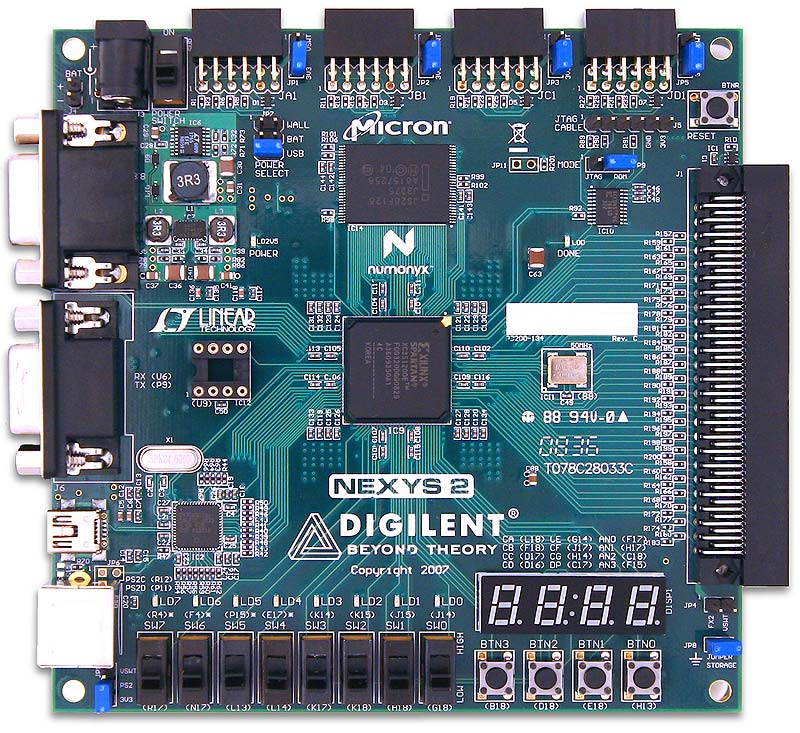
\includegraphics[width=0.7\textwidth]{model}
 \caption{Modelo de la Nexxys , Versión 2.}
    \label{fig:btn}
\end{figure}
  
 Algunas de las que mas nos llamaron la atencion son :
  \item[Caracteristicas] \hfill \\
    	\begin{itemize}
			\item Xilinx Spartan-3E FPGA 500K
			\item Memoria PSDRAM de 16 MB fast Micron® 
			\item Memoria de 16 MB Intel® StrataFlash® Flash R 
      		\item Trabaja con la version Free de ISE®/WebPACK 
            \item Oscillador de 50 MHz
			\item Fuentes reguladas de 3.3V@3A/100mA(principal),3.3V@150mA/60mA,2.5V/1.2V@1.4A/50mA
            \item Todas las entradas tiene protección contra cortocircuitos y descargas electroestatica
  			\item Incluye  8 leds, cuatro display siete segmentos, cuatro pulsadores, 8 switches four pushbuttons, eight slide switches
      \end{itemize}
      entre otras\ldots
\end{description}
Para plantear una solución al problema mencionado en \ref{sec:problemamecanico}, nosotros hemos descargado el esquemático para comprender circuitalmente cuál es la configuración de los pulsadores, aunque generalmente para desarrollos importantes en electrónica, se compran  pulsadores de alta calidad, y resistencia mecánica a presiones momentaneas e instántaneas, pero dado que esto es una placa de entrenamiento, \textit{estudiantil} asumimos que los pulsadores que esta posee son netamente mecánicos que cuenta con el diseño de la figura \ref{fig:btn}

\begin{figure}[!ht]
  \centering
     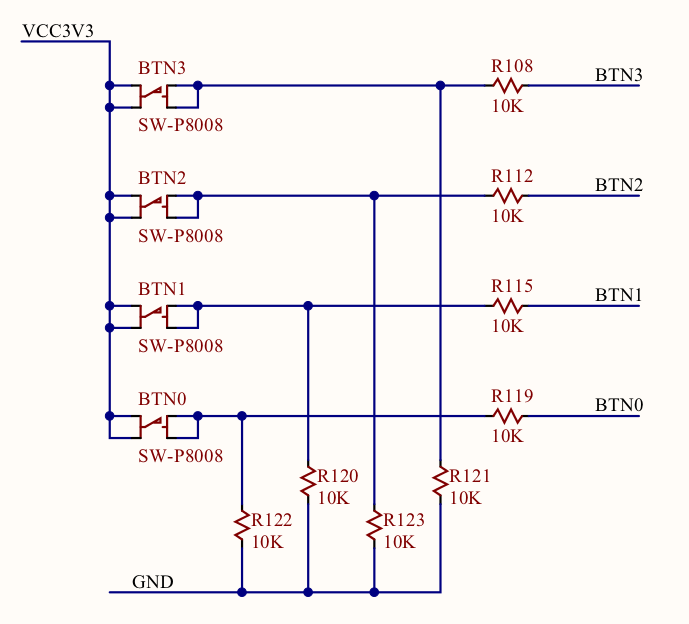
\includegraphics[width=0.7\textwidth]{btn1.png}
  \caption{Esquema provisto en el esquematico, 4 pulsadores.}
    \label{fig:btn}
\end{figure}

\begin{figure}[!ht]
  \centering
     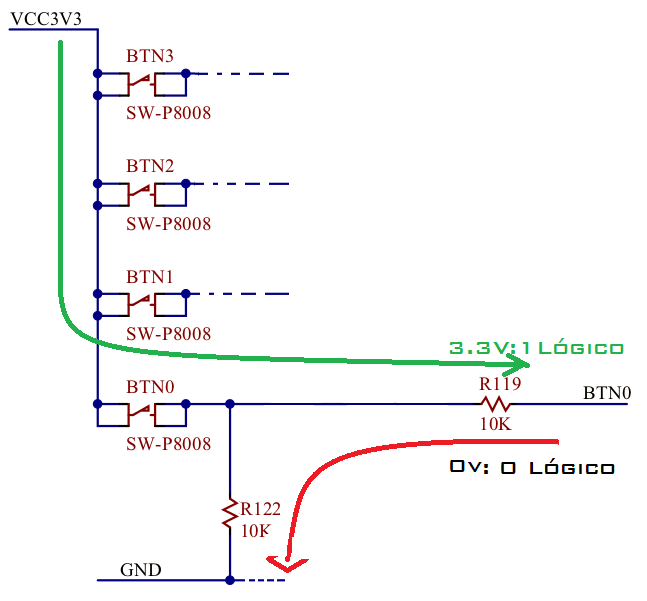
\includegraphics[width=0.7\textwidth]{btn2.png}
  \caption{Circulación de la corriente en el circuito, resistencia de 10k protección contra cortocircuito}
      \label{fig:btn2}
\end{figure}
La figura \ref{fig:btn2} también muestra una configuración de un solo pulsador vemos la resistencia de pull down. Con colores hemos indicado el accionamiento del pulsador, tome como ejemplo \ref{fig:btn2}, el color rojo indica cuando el pulsador \textbf{BTN0} no ha sido presionado, esto indica que los pulsadores son de tipo \textbf{N.O} ó \textit{Normally Open} presentando un \textbf{0 lógico} a la salida, al presionar el pulsador, el contacto interno que este posee cierra el circuito conectándolo con la fuente de 3.3v como lo muestra el color verde.
\section{Explicación Código VHDL}
This is some VHDL code: we need to describe it very carefully and in a detail form.
\begin{minted}{vhdl}
process
begin
  CLK <= '1'; wait for 10 NS;
  CLK <= '0'; wait for 10 NS;
end process;
\end{minted}
Codigo de Ejemplo de Anti-Rebote.
\inputminted{vhdl}{./Code/debounce.vhd}

\section{Prácticas Experimentales}
Poner a qui la practica realizada en laboratorio.

\end{document}